\chapter{Results}
\label{ch_results}

%These are the results I found from my investigation.

%Present your results in a suitable format using tables and graphs where necessary. Remember to refer to them in text and caption them properly.

\section{Experimental Results}

\subsection{Focal Length of Lens}

The measured focal length of the lens was measured to be 53mm. Figure \ref{fig:focal_length_experiemnt_result} shows the focused point formed after adjusting the lens to 5.3cm above the working surface.

\begin{figure}[H]
	\centering
	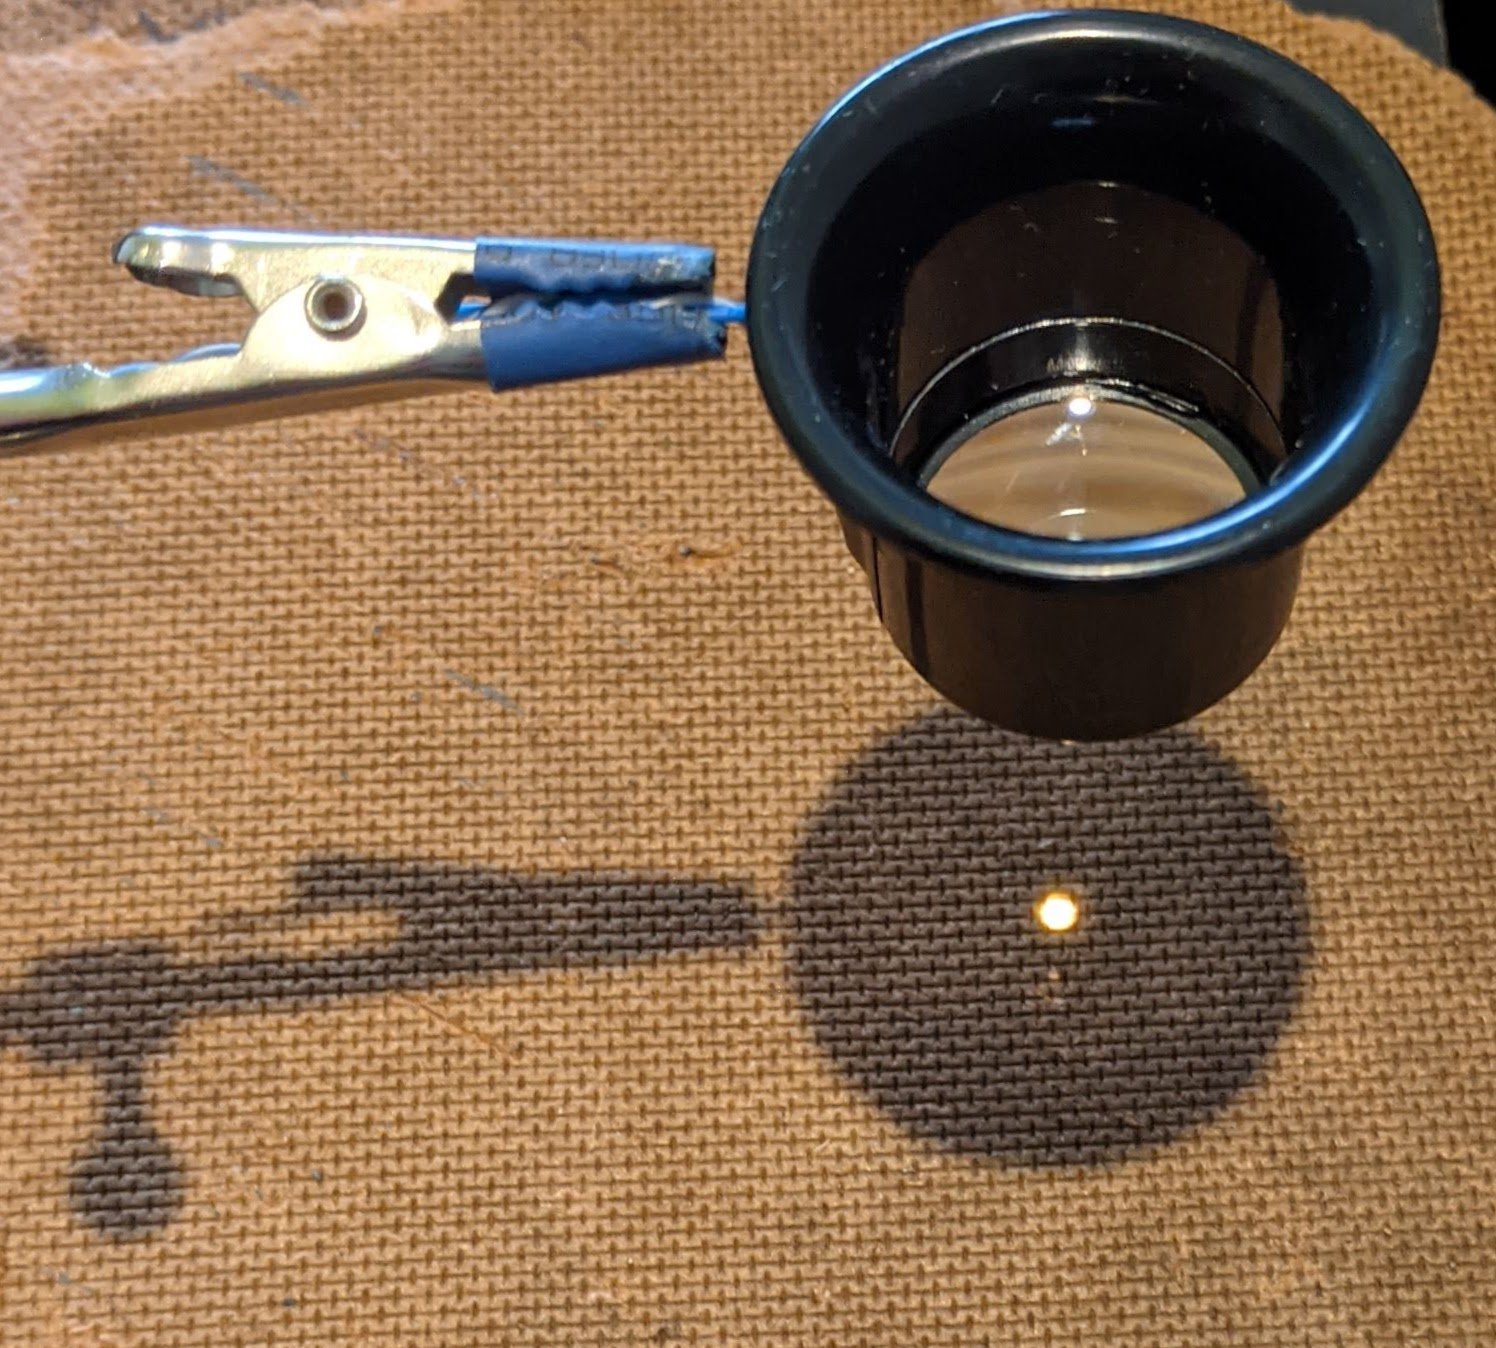
\includegraphics[width=.6\linewidth]{figures/results/focal_length_result.jpg}
	\captionof{figure}{Focal Length Experiemnt}
	\label{fig:focal_length_experiemnt_result}
\end{figure}


\subsection{IR Beam Dispersion}

\begin{figure}[H]
	\centering
	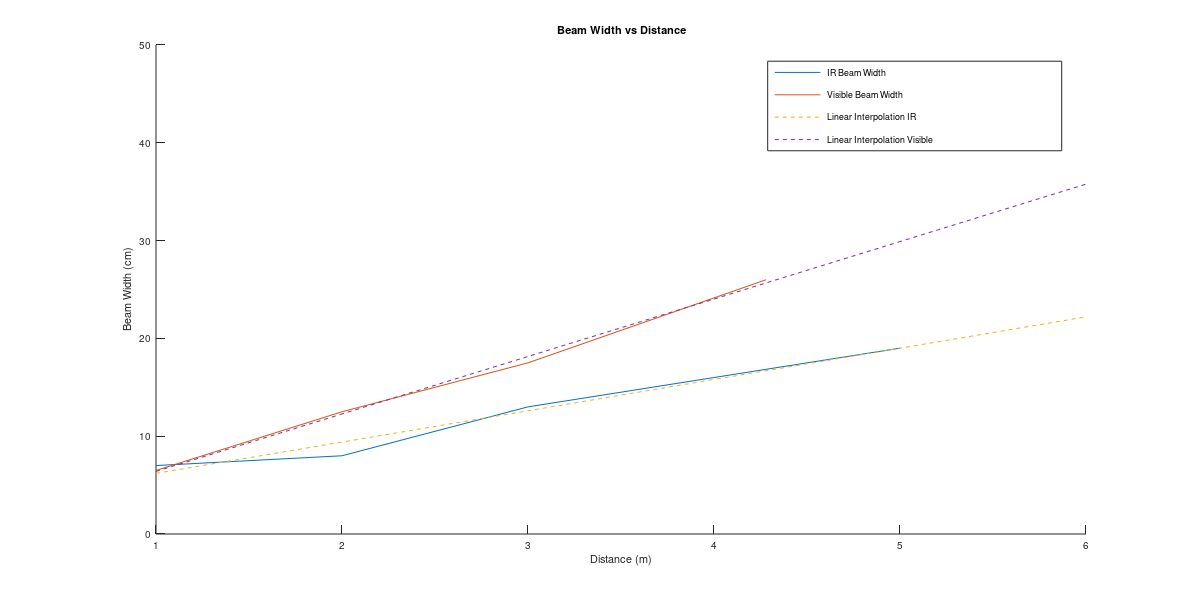
\includegraphics[width=\linewidth]{figures/results/beam_width_vs_distance.png}
	\captionof{figure}{Beam Width vs Distance}
	\label{fig:beam_width_vs_distance}
\end{figure}



%todo: ref this table
Table \ref{tbl:spot_size_vs_distance} below shows the beam spot size vs distance for the IR and white power LEDs.

%todo: update these images
\begin{figure}[H]
	\centering
	\begin{minipage}{.4\textwidth}
		%todo: make image higher quality after zoom
		\textbf{Linear Interpolation Equations}
		
		\[width_{ir\: beam} = 0.03 + 0.032 \times d_{beam}\]
		
		\[width_{visible\: beam} = 0.00526 + 0.0587 \times d_{beam}\]
		
		
	\end{minipage}%
	\hspace{.1\textwidth}
	\begin{minipage}{.4\textwidth}
		\begin{table}[H]
			\begin{tabular}{ccc}
				\hline
				\textbf{\begin{tabular}[c]{@{}c@{}}Distance\\ (m)\end{tabular}} & \textbf{\begin{tabular}[c]{@{}c@{}}IR Beam\\ Width\\ (cm)\end{tabular}} & \textbf{\begin{tabular}[c]{@{}c@{}}Visible Beam\\ Width\\ (cm)\end{tabular}} \\ \hline
				1 & 7 & 6.5 \\ \hline
				2 & 8 & 12.5 \\ \hline
				3 & 13 & 17.5 \\ \hline
				4 & 16 & - \\ \hline
				4.28 & - & 26 \\ \hline
				5 & 19 & - \\ \hline
			\end{tabular}
			\captionof{table}{Tabulation of Spot Diameter V.S. Distance}
			\label{tbl:spot_size_vs_distance}
		\end{table}
	\end{minipage}
\end{figure}

\subsection{Goertzel Filter Benchmark}

The results from the goertzel algorithm optimization experiment are tabulated in table \ref{tbl:goertzel_speed_results}, the adjacent screenshot shown in figure \ref{fig:goertzel_speed_scope_screenshot} illustrates the output recorded by the oscilloscope software during a single iteration of the experiment. 

\begin{figure}[H]
	\centering
	\begin{minipage}{.4\textwidth}
		%todo: make image higher quality after zoom
		\centering
		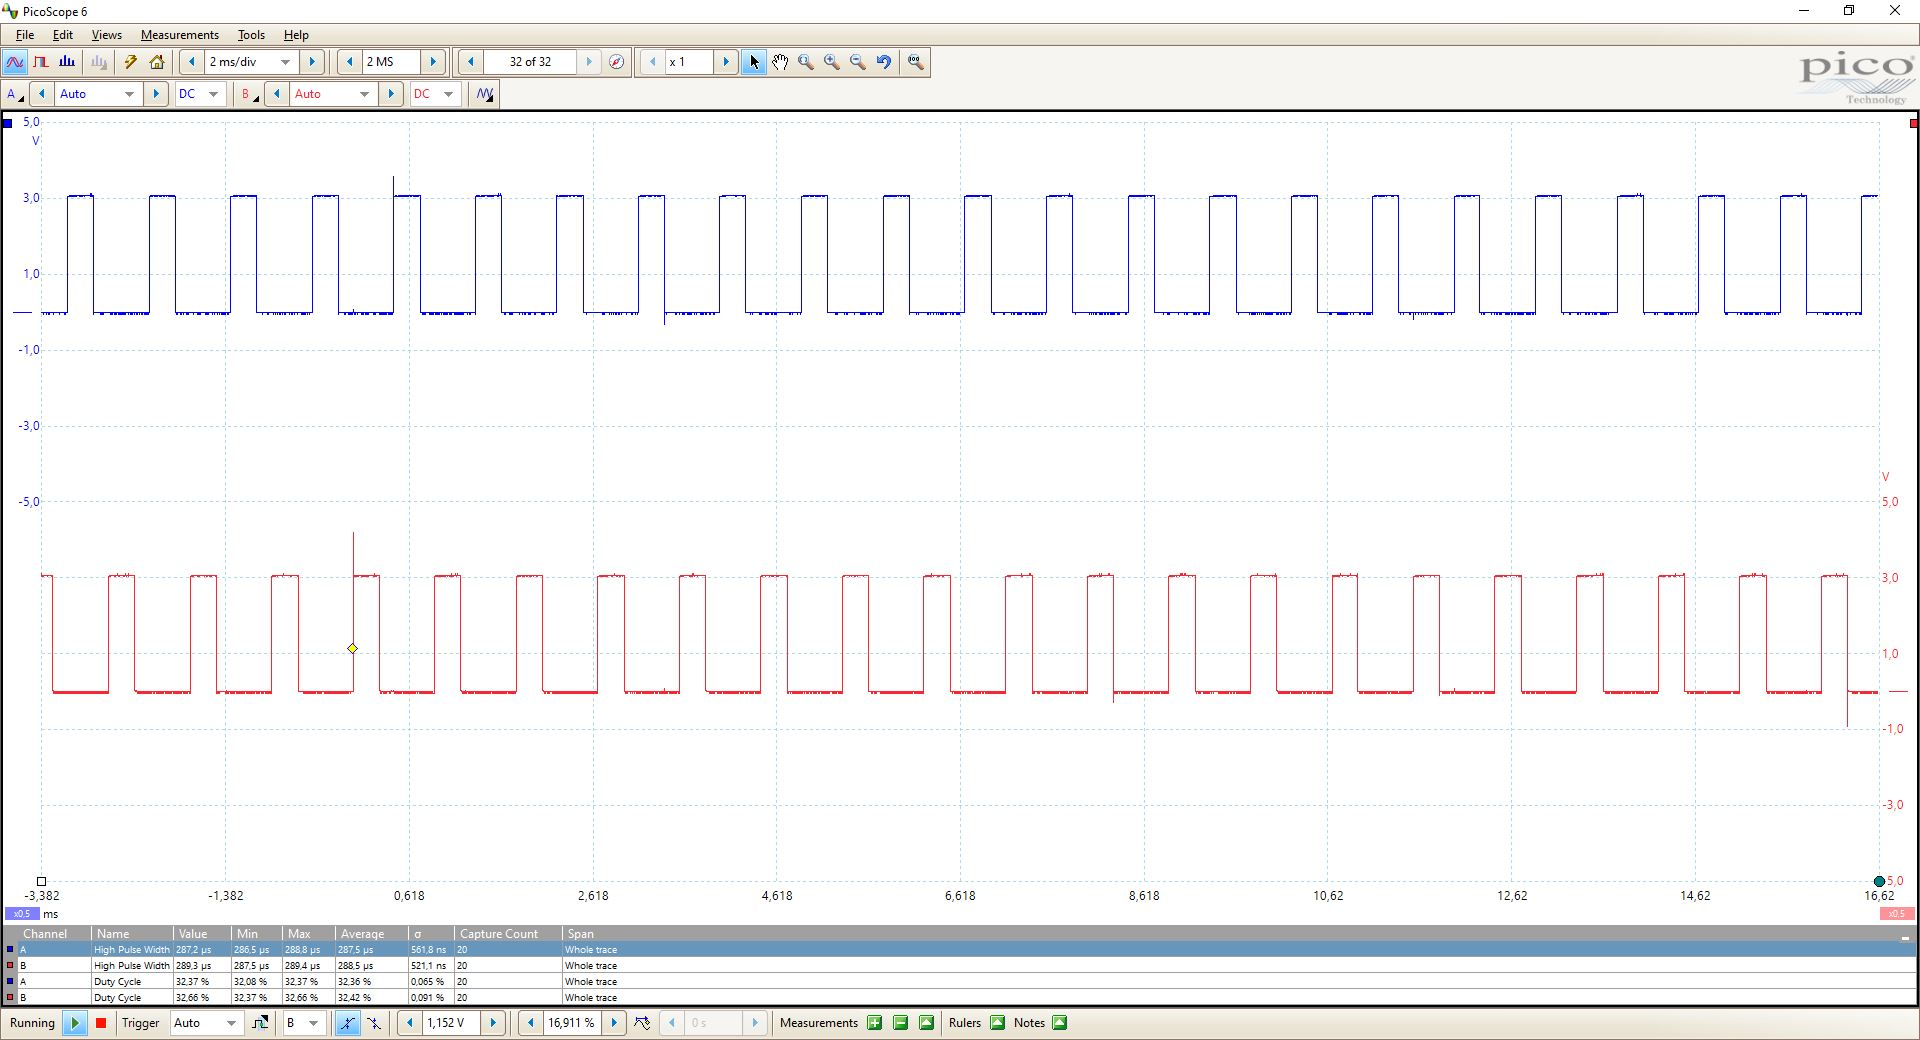
\includegraphics[width=0.9\linewidth]{figures/results/goertzel_filter_speed/16nu.JPG}
		\captionof{figure}{Scope Reading for unoptimized goertzel with $N = 16$}
		\label{fig:goertzel_speed_scope_screenshot}
	\end{minipage}%
	\hspace{.1\textwidth}
	\begin{minipage}{.4\textwidth}
		\begin{table}[H]
			\begin{tabular}{ccc}
				\hline
				\textbf{N} & \textbf{\begin{tabular}[c]{@{}c@{}}Unoptimized\\ ($\mu S$)\end{tabular}} & \textbf{\begin{tabular}[c]{@{}c@{}}Optimized\\ ($\mu S$)\end{tabular}} \\ \hline
				4 & 96.46 & 61.15 \\ \hline
				8 & 160.3 & 98.35 \\ \hline
				16 & 287.5 & 171.9 \\ \hline
				32 & 547.2 & 323.9 \\ \hline
				64 & 1059 & 621.1
			\end{tabular}
			\captionof{table}{Compiled results for goertzel speed experiemnt}
			\label{tbl:goertzel_speed_results}
		\end{table}
	\end{minipage}
\end{figure}

The recorded results are plotted in figure \ref{fig:goertzel_computation_plot} to provide graphical insight.

\begin{figure}[H]
	\centering
	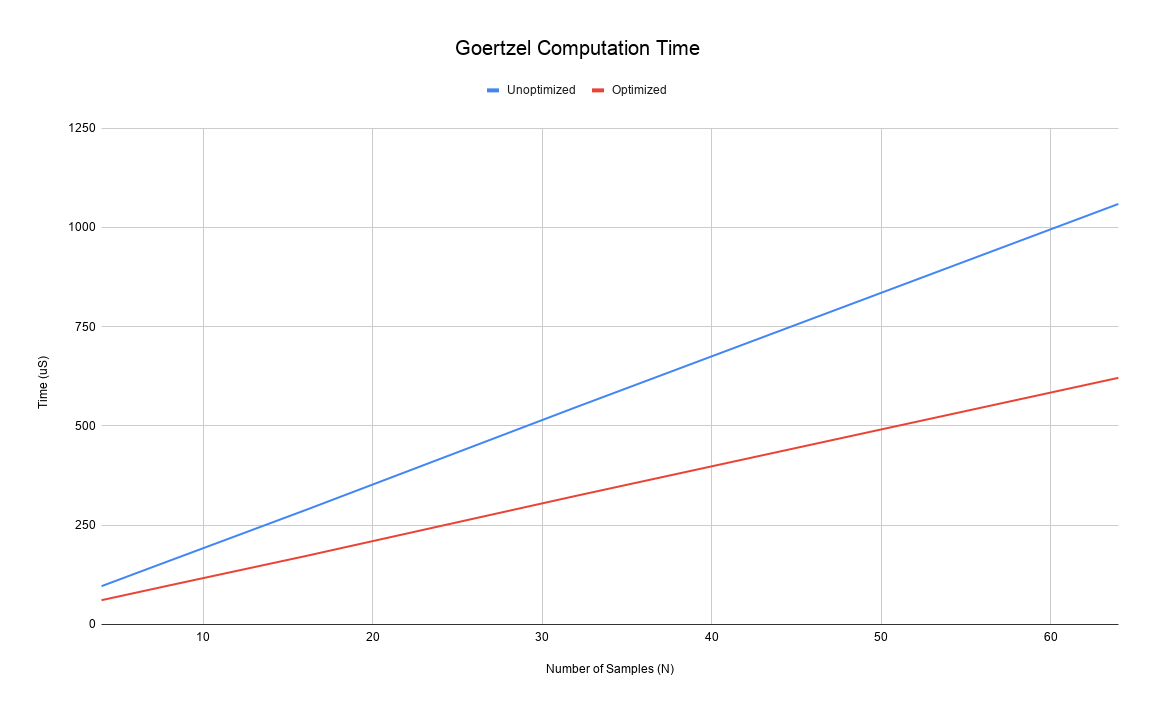
\includegraphics[width=\linewidth]{figures/results/goertzel_filter_speed/goertzel_computation_time.png}
	\captionof{figure}{Goertzel computation time versus sample set size}
	\label{fig:goertzel_computation_plot}
\end{figure}

%disc. removed

\subsection{Goertzel Filter Performance}

\subsubsection{Simulated Frequency Response}

%disc. removed

\begin{figure}[H]
	\centering
	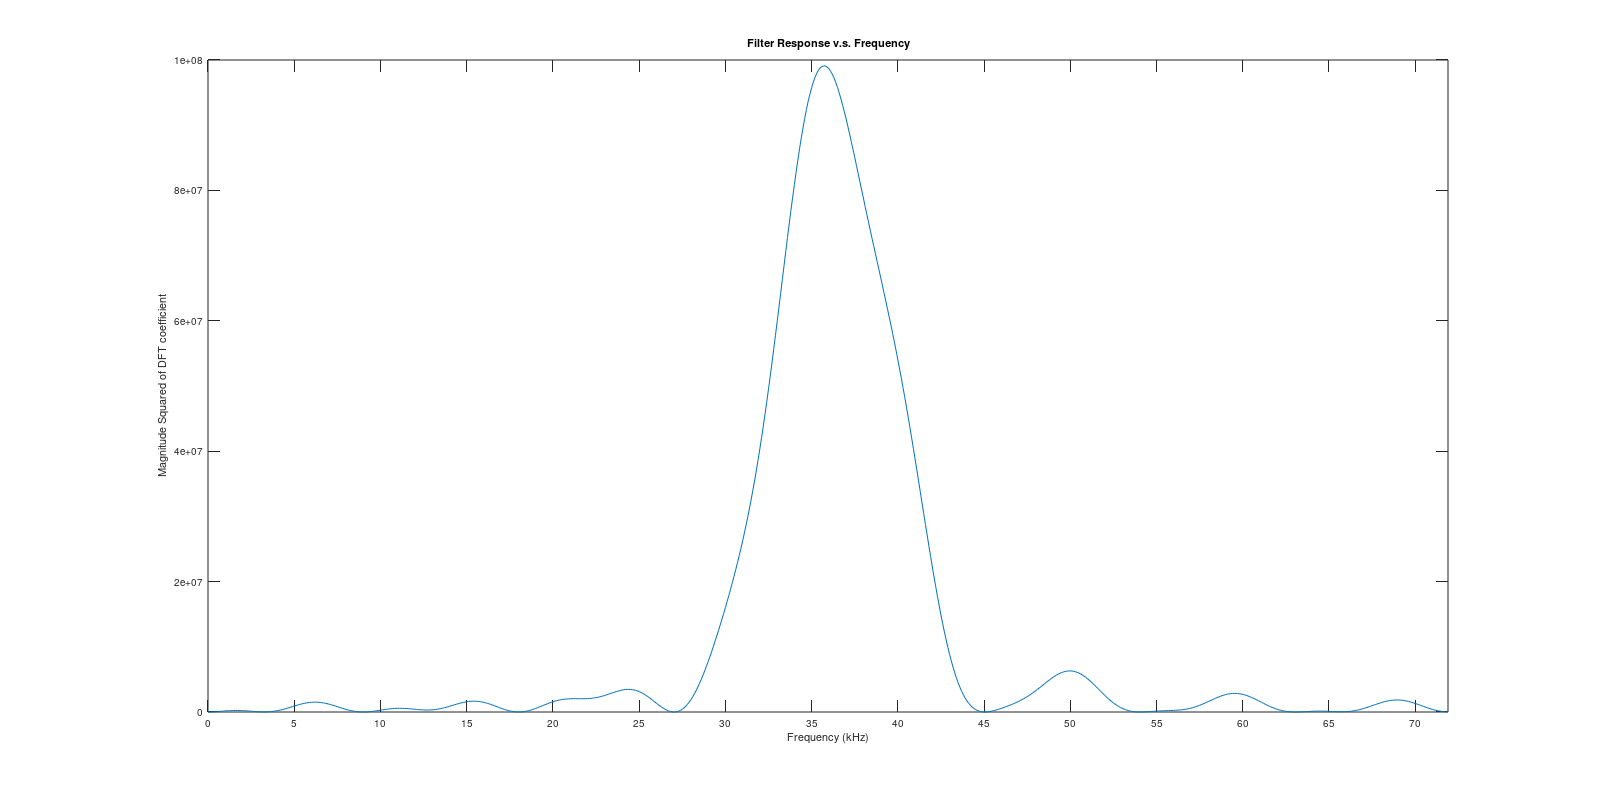
\includegraphics[width=\linewidth]{figures/results/goertzel_filter_simulation_wide.png}
	\caption{Expected Frequency Response - Goertzel Filter}
	\label{fig:goertzel_filter_response_simulated}
\end{figure}

%disc. removed

\subsubsection{Measured Frequency Response}

The following plot in figure \ref{fig:goertzel_filter_response_empirical} show the values returned by the Goertzel filter module and shows the expected frequency response curve.

\begin{figure}[H]
	\centering
	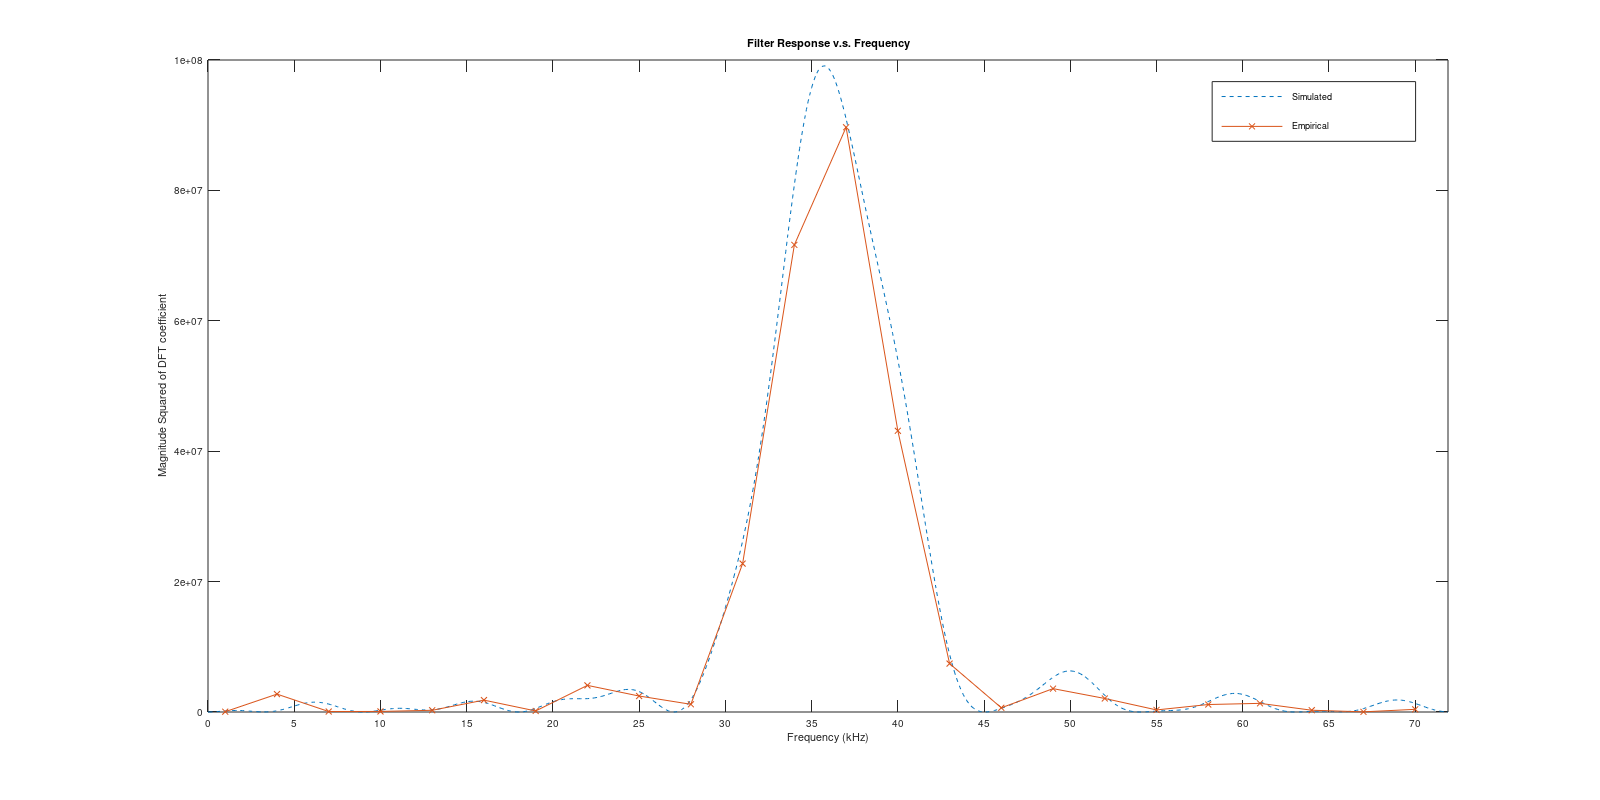
\includegraphics[width=\linewidth]{figures/results/goertzel_filter_empirical_wide.png}
	\caption{Measured Frequency Response - Goertzel Filter}
	\label{fig:goertzel_filter_response_empirical}
\end{figure}

\subsubsection{Trigger Conditions}

\begin{table}[H]
	\centering
	\begin{tabular}{ccc}
		\hline
		\begin{tabular}[c]{@{}c@{}}Amplitude\\ (mV)\end{tabular} & \begin{tabular}[c]{@{}c@{}}Trigger Frequency\\ Lower (kHz)\end{tabular} & \begin{tabular}[c]{@{}c@{}}Trigger Frequency\\ Upper (kHz)\end{tabular} \\ \hline
		297 & 35.12 & 36.79 \\ \hline
		300 & 34.7 & 37.23 \\ \hline
		350 & 32.74 & 39.27 \\ \hline
		400 & 31.86 & 40.16 \\ \hline
		450 & 31.29 & 40.78 \\ \hline
		500 & 30.86 & 41.2 \\ \hline
	\end{tabular}
	\captionof{table}{Amplitude-Voltage Boundry Pairs}
	\label{tbl:amplitude_voltage_trigger_pairs}
\end{table}

\begin{figure}[H]
	\centering
	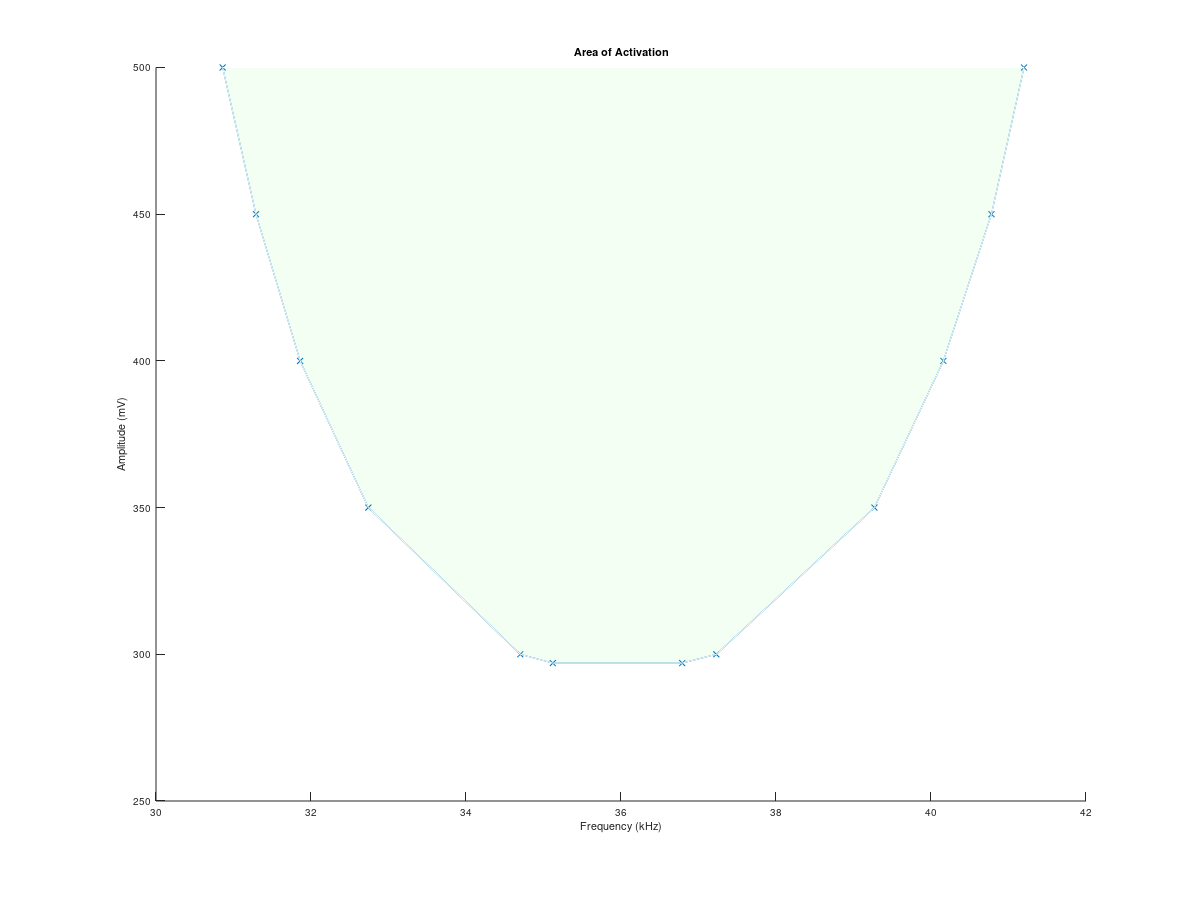
\includegraphics[width=.8\textwidth]{figures/results/goertzel_amplitude_frequency_pairs.png}
	\captionof{figure}{Area of Sensitivity Goertzel Filter}
	\label{fig:goertzel_amplitude_frequency_pairs}
\end{figure}


\subsection{Carrier Waveform Generation Performance}
%todo: this



\subsection{Power LED Driver Performance}

The following screenshots shown in figures \ref{fig:pwr_led_6k} through \ref{fig:pwr_led_96k} show the results captured by the oscilloscope. The red trace shows the output of the function generator and the blue trace shows the voltage across the shunt resistor R1\footnote{see schematic in figure \ref{fig:schematic_power_led_driver}}.

\begin{figure}[H]
	\centering
	\begin{minipage}{.399\linewidth}
		\centering
		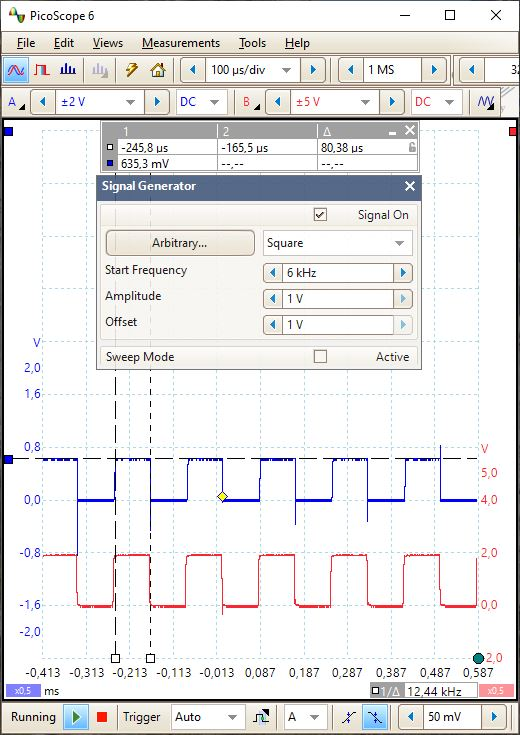
\includegraphics[width=\textwidth]{figures/results/power_led_driver/6khz.JPG}
		\captionof{figure}{6kHz Driving Frequency}
		\label{fig:pwr_led_6k}
	\end{minipage}%
	\hspace{.1\linewidth}
	\begin{minipage}{.399\linewidth}
		\centering
		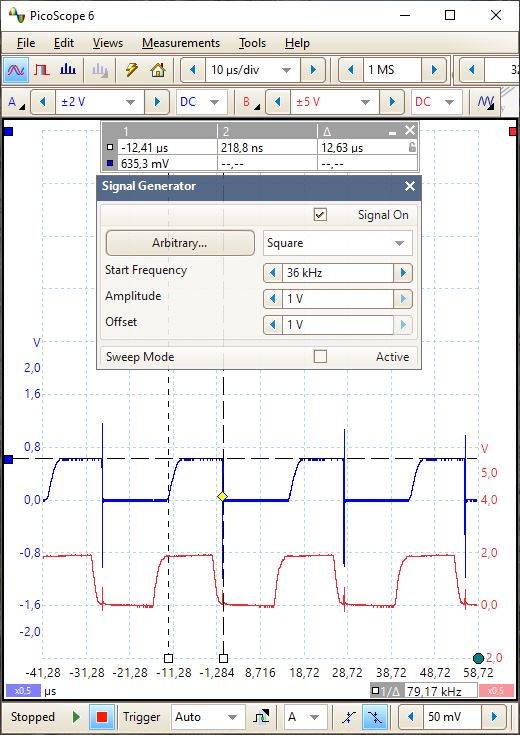
\includegraphics[width=\textwidth]{figures/results/power_led_driver/36khz.JPG}
		\captionof{figure}{36kHz Driving Frequency}
		\label{fig:pwr_led_36k}
	\end{minipage}
\end{figure}

\begin{figure}[H]
	\centering
	\begin{minipage}{.4\linewidth}
		\centering
		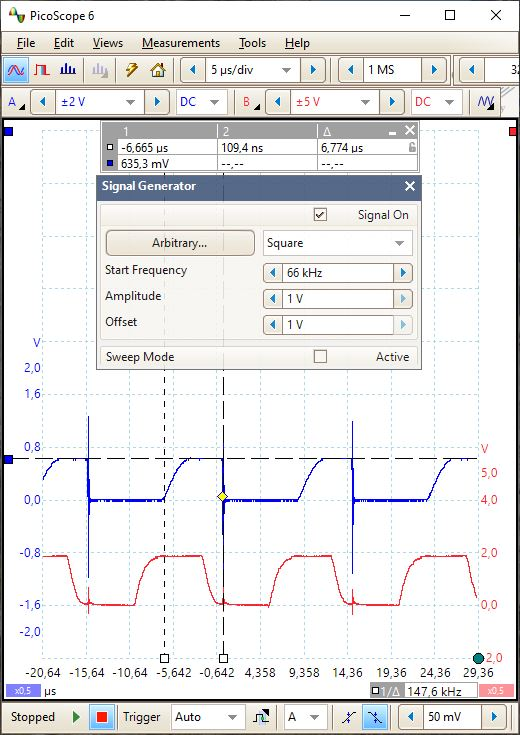
\includegraphics[width=\textwidth]{figures/results/power_led_driver/66khz.JPG}
		\captionof{figure}{66kHz Driving Frequency}
		\label{fig:pwr_led_66k}
	\end{minipage}
	\hspace{.1\linewidth}
	\begin{minipage}{.4\linewidth}
		\centering
		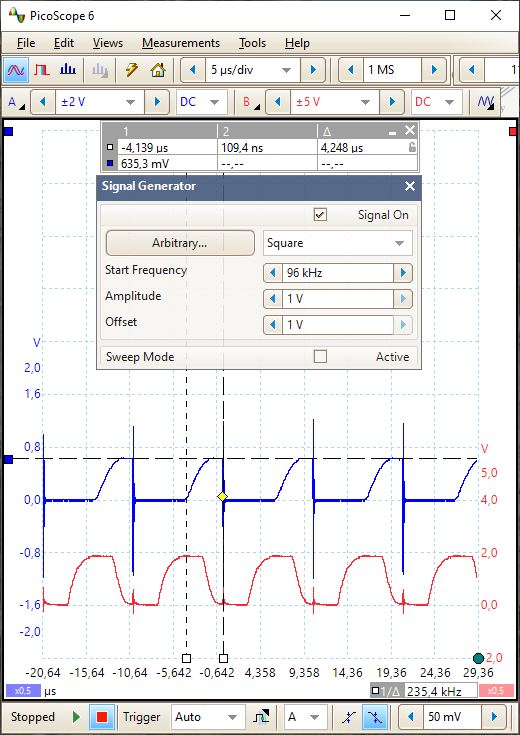
\includegraphics[width=\textwidth]{figures/results/power_led_driver/96khz.JPG}
		\captionof{figure}{96kHz Driving Frequency}
		\label{fig:pwr_led_96k}
	\end{minipage}
\end{figure}

\begin{table}[H]
	\centering
	\begin{tabular}{ccc}
		\hline
		\textbf{\begin{tabular}[c]{@{}c@{}}Frequency\\ (kHz)\end{tabular}} & \textbf{\begin{tabular}[c]{@{}c@{}}LED Current\\ (mA)\end{tabular}} & \textbf{\begin{tabular}[c]{@{}c@{}}Duty Cycle\\ (\%)\end{tabular}} \\ \hline
		6 & 908 & 48.2 \\ \hline
		36 & 908 & 45.5 \\ \hline
		66 & 908 & 44.7 \\ \hline
		96 & 908 & 40.8 \\ \hline
	\end{tabular}
	\caption{Frequency V.S. Current and Pulse Width}
	\label{tbl:led_driver_tabulated_results}
\end{table}



\subsection{Directivity of IR Modules}

Figure \ref{fig:vrms_vs_angle_of_incidence} shows the RMS voltage value of the modules output with respect to the angle of incidence. Figure \ref{fig:beam_pattern} shows the normalized RMS voltage value and mirrors the image about the vertical to provide an illustration of the beam pattern.


\begin{figure}[H]
	\centering
	\begin{minipage}{.4\linewidth}
		\centering
		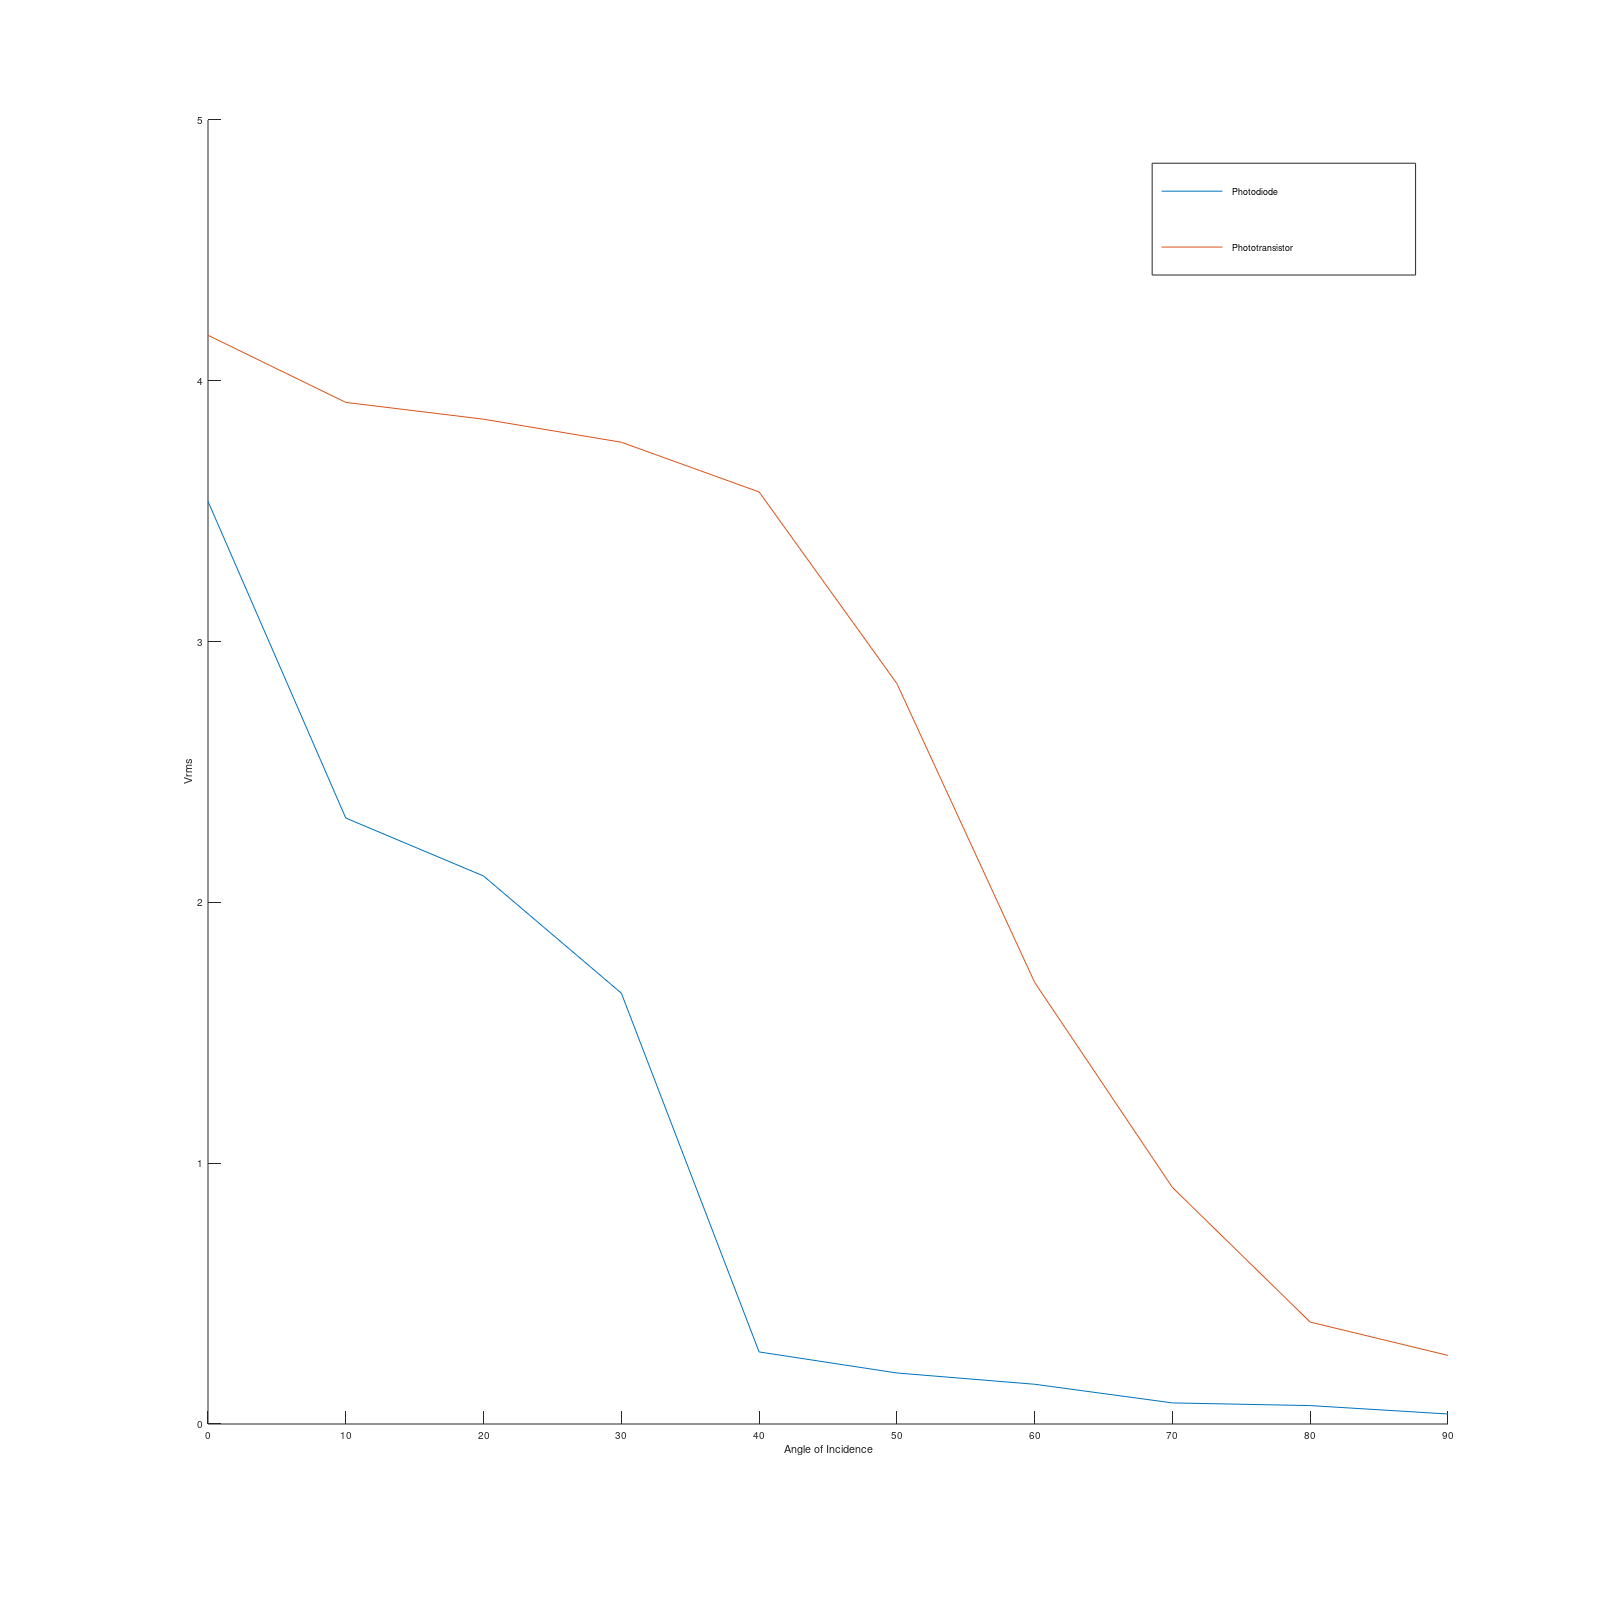
\includegraphics[width=\textwidth]{figures/results/vrms_vs_incidence_square.png}
		\captionof{figure}{Vrms vs Angle of Incidence}
		\label{fig:vrms_vs_angle_of_incidence}
	\end{minipage}
	\hspace{.1\linewidth}
	\begin{minipage}{.4\linewidth}
		\centering
		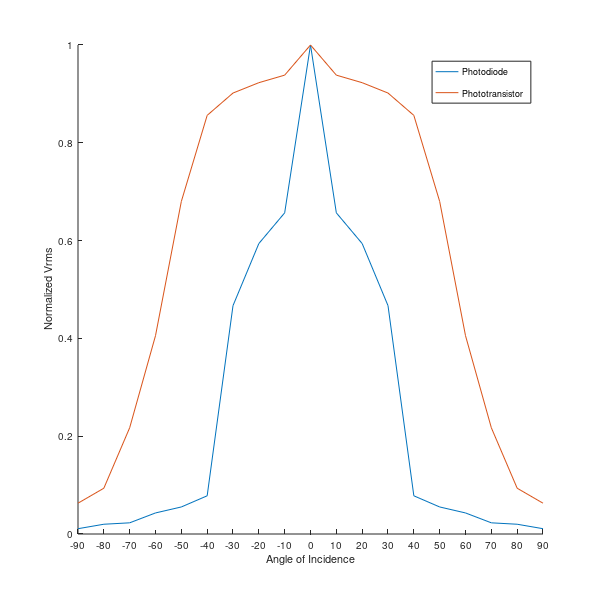
\includegraphics[width=\textwidth]{figures/results/beam_pattern_square.png}
		\captionof{figure}{Beam Pattern}
		\label{fig:beam_pattern}
	\end{minipage}
\end{figure}

The IR receiver module registered the signal between angles of 0\textdegree and 70\textdegree and registered an absence of a signal for angles greater than 80\textdegree. Between 70\textdegree and 80\textdegree the output would toggle sporadically.


\subsection{Target MCU Performance}

\subsubsection{Processing Time}

\begin{figure}[H]
	\centering
	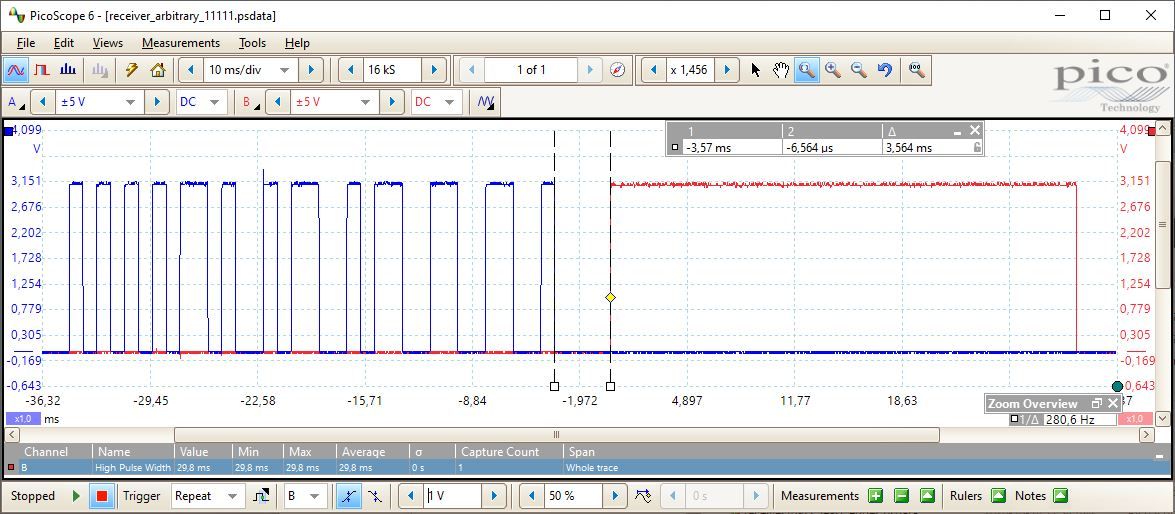
\includegraphics[width=.8\textwidth]{figures/results/receiver_software/arbitrary_11111_timing_test.JPG}
	\caption{Oscilloscope Trace for Transmission of 11111}
	\label{fig:arbitrary_11111_timing_test}
\end{figure}

\begin{table}[H]
	\centering
	\begin{tabular}{cccc}
		\hline
		\textbf{\begin{tabular}[c]{@{}c@{}}15-Bit Data\\ (Decimal)\end{tabular}} & \textbf{Number of Edges} & \textbf{\begin{tabular}[c]{@{}c@{}}Timeout Delay\\ (ms)\end{tabular}} & \textbf{\begin{tabular}[c]{@{}c@{}}Decoding Time\\ (ms)\end{tabular}} \\ \hline
		10922 & 20 & 3.56 & 29.7 \\ \hline
		11111 & 26 & 3.56 & 29.8 \\ \hline
		32767 & 36 & 3.56 & 29.9 \\ \hline
	\end{tabular}
\end{table}

Combining the timeout delay and decoding time gives a maximum period of 33.46ms in the worst case, before a new message may be received.

\subsection{System Performance}